\byline{{\textbf{\Large\sffamily December Bonsai Club Meetup:}}\\
{\textbf{\large\sffamily Festive Spirits and Focused Learning}}}{The Newsletter Team}
\noindent
As our final meeting of the year, the atmosphere was wonderfully relaxed, with members bringing along drinks and snacks to kick off the festive season.

While some faced delays getting to the venue, others unfortunately dealt with more serious setbacks that prevented them from attending.
We send our most sincere wishes for a \textbf{speedy recovery} to those who were unable to join us; you were certainly missed.

Despite a slightly lower turnout than usual, it remained a highly productive evening.
Our \textbf{Tree of the Month} competition featured several creative, Christmas-themed entries from both Novice and General members (see p.~\pageref{2025-12-totm}).
Meanwhile, the workshop was buzzing with activity as members worked on a diverse range of specimens, from youthful small starters to mature large trees.

\medskip
The evening also served as a perfect lead\--in to our new \textbf{Member Education Programme (MEP)}.
For those unfamiliar with the initiative, these sessions allow our more experienced members to mentor newer practitioners.
To support this, the club fully covers the booking costs for the venue's front room on the selected Saturday mornings.

The next session on \textbf{Saturday, 13th December} will focus on \textbf{wiring and winter pruning}, see p.~\pageref{2025-12-workshop-mep} for further details and a report of the event.
The following session on \textbf{Saturday, 17th January 2026} will be dedicated to \textbf{repotting and root pruning} and due to high interest, the committee has already scheduled another one on \textbf{Saturday, 28th February 2026} again on \textbf{repotting and positioning within the container}.
If you would like to attend, please contact \textbf{Tony Ulatowski} or \textbf{Chris Durne} via WhatsApp to secure your spot, as they are being snapped up fast!

\medskip
We wish you all a fantastic holiday break and look forward to seeing you refreshed and ready for the new year in January.

\medskip
\vspace*{-1em}
\begin{window}[2,l,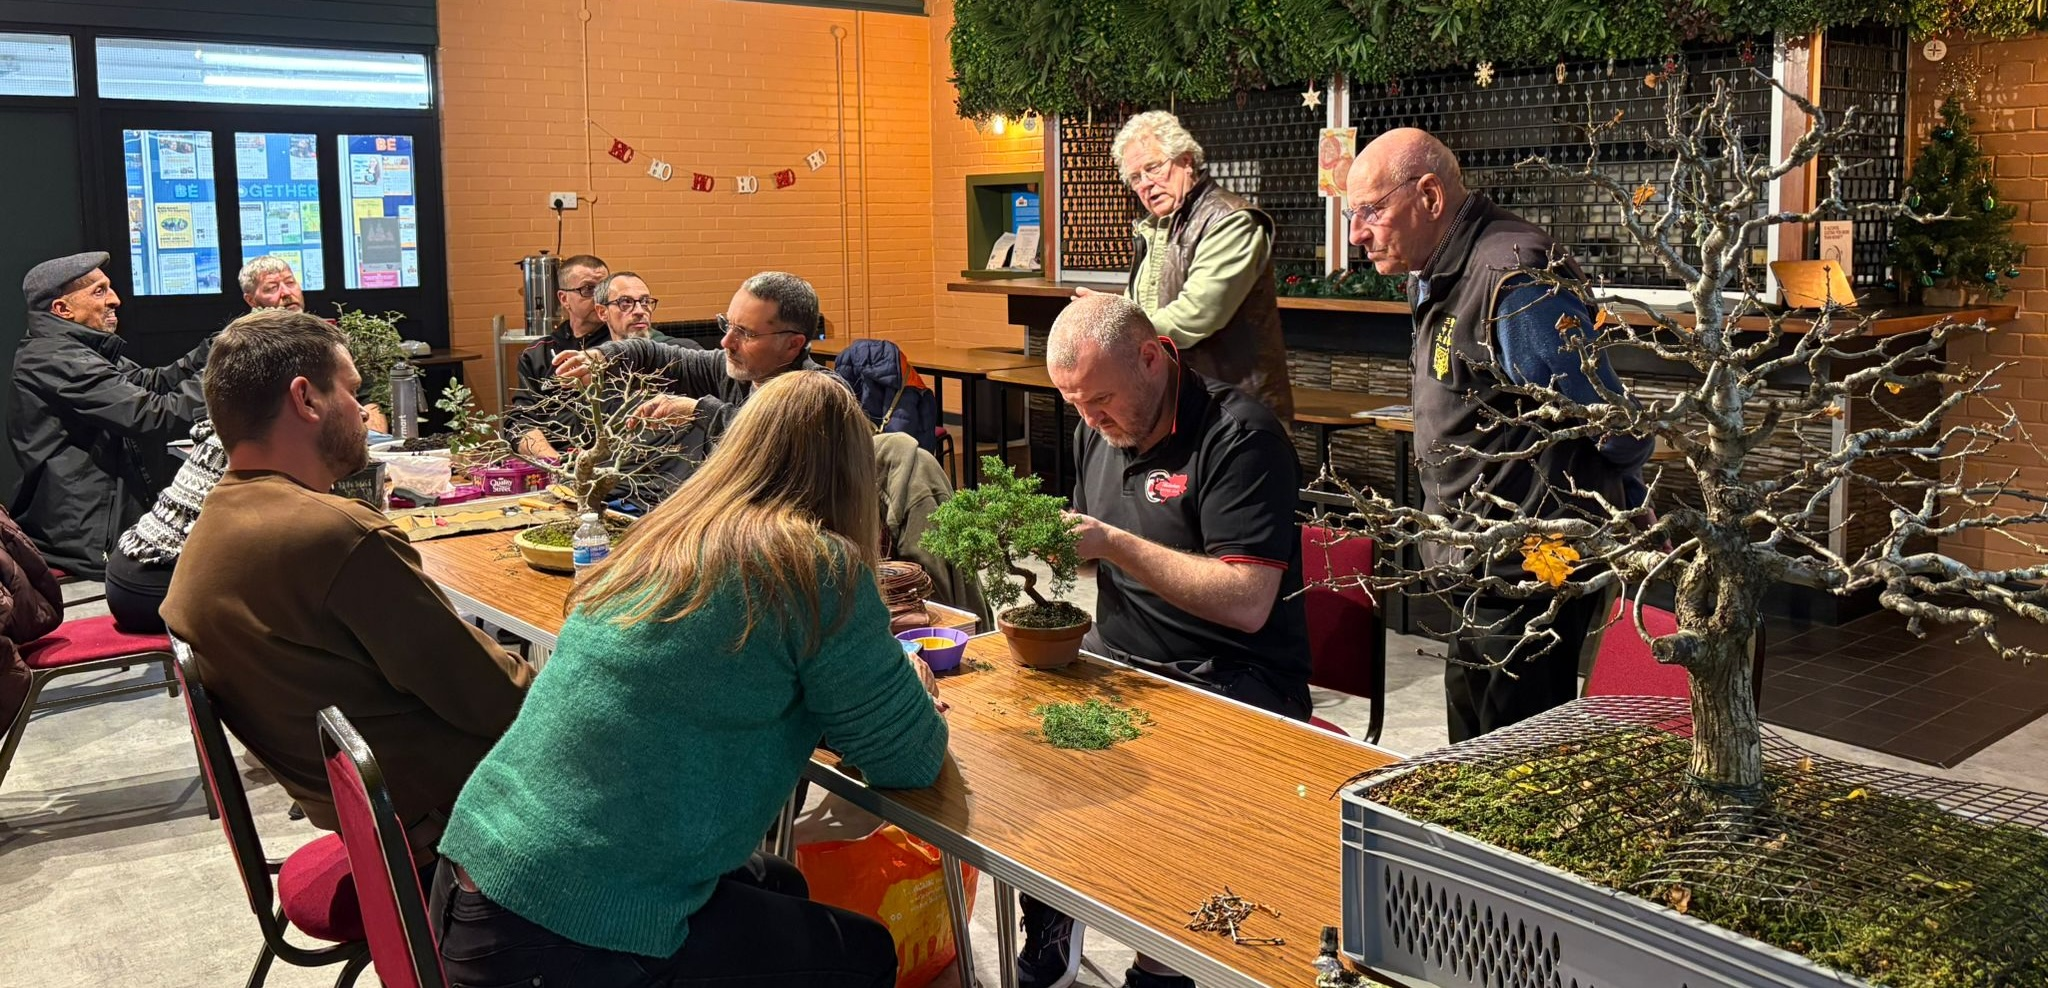
\includegraphics[width=1.0\columnwidth]{2025_12/res/editorial_december},\centerline{\emph{Members enjoying the festive workshop atmosphere.}}]
\end{window}
\vspace*{-1em}
\closearticle
\clearpage


%\byline{{\textbf{\Large\sffamily December Bonsai Club Meetup:}}\\
%{\textbf{\large\sffamily Festive Spirits and Focused Learning}}}{The Newsletter Team}
%\noindent
%As our final meeting of the year, the evening was defined by a wonderfully relaxed atmosphere. Members brought along a variety of drinks and snacks to kick off the festive season, making for a very sociable start to the holidays.
%
%While some faced minor delays getting to the venue, others unfortunately dealt with more serious setbacks that prevented them from attending. We send our very most sincere wishes for a \textbf{speedy recovery} to those who were unable to join us; you were certainly missed.
%
%Despite a slightly lower turnout than usual as a result, it remained a highly active and productive evening. We held our regular \textbf{Tree of the Month} competition for both Novice and General members, which featured several creative, Christmas-themed entries that brought a bit of seasonal magic to the display tables. For a full look at the winners, see the article at p.~\pageref{contest}.
%
%\medskip
%The workshop portion of the evening was particularly vibrant. Many members brought trees to work on, ranging from youthful starters to impressive mature specimens. It was a pleasure to see the room filled with such a diverse range of sizes and species, making for a truly hands-on session.
%
%\medskip
%The meeting also served as a great lead-in to the launch of our new \textbf{Member Education Programme (MEP)}. For those who haven't yet heard, the MEP pairs our more experienced members with newer practitioners for dedicated mentoring. These sessions are held on \textbf{Saturday mornings} in the front room of our usual venue, with the room booking fully covered by the club to ensure everyone can participate.
%
%The next session is scheduled for \textbf{Saturday, 17th January}, focusing on \textbf{wiring and winter pruning} as we prepare for the repotting season. Given the high level of interest, the committee has already added a February date to the calendar specifically for \textbf{repotting, root pruning, and wiring}.
%
%If you would like to secure a place, please contact \textbf{Tony Ulatowski} via WhatsApp as soon as possible—spots are being snapped up fast! More details on the MEP can be found at p.~\pageref{mep-details}.
%
%\medskip
%We wish you all a wonderful holiday break and look forward to seeing you—and your trees—refreshed and ready for the new year in January.
%\medskip
%
%\vspace*{-1em}
%\begin{window}[2,l,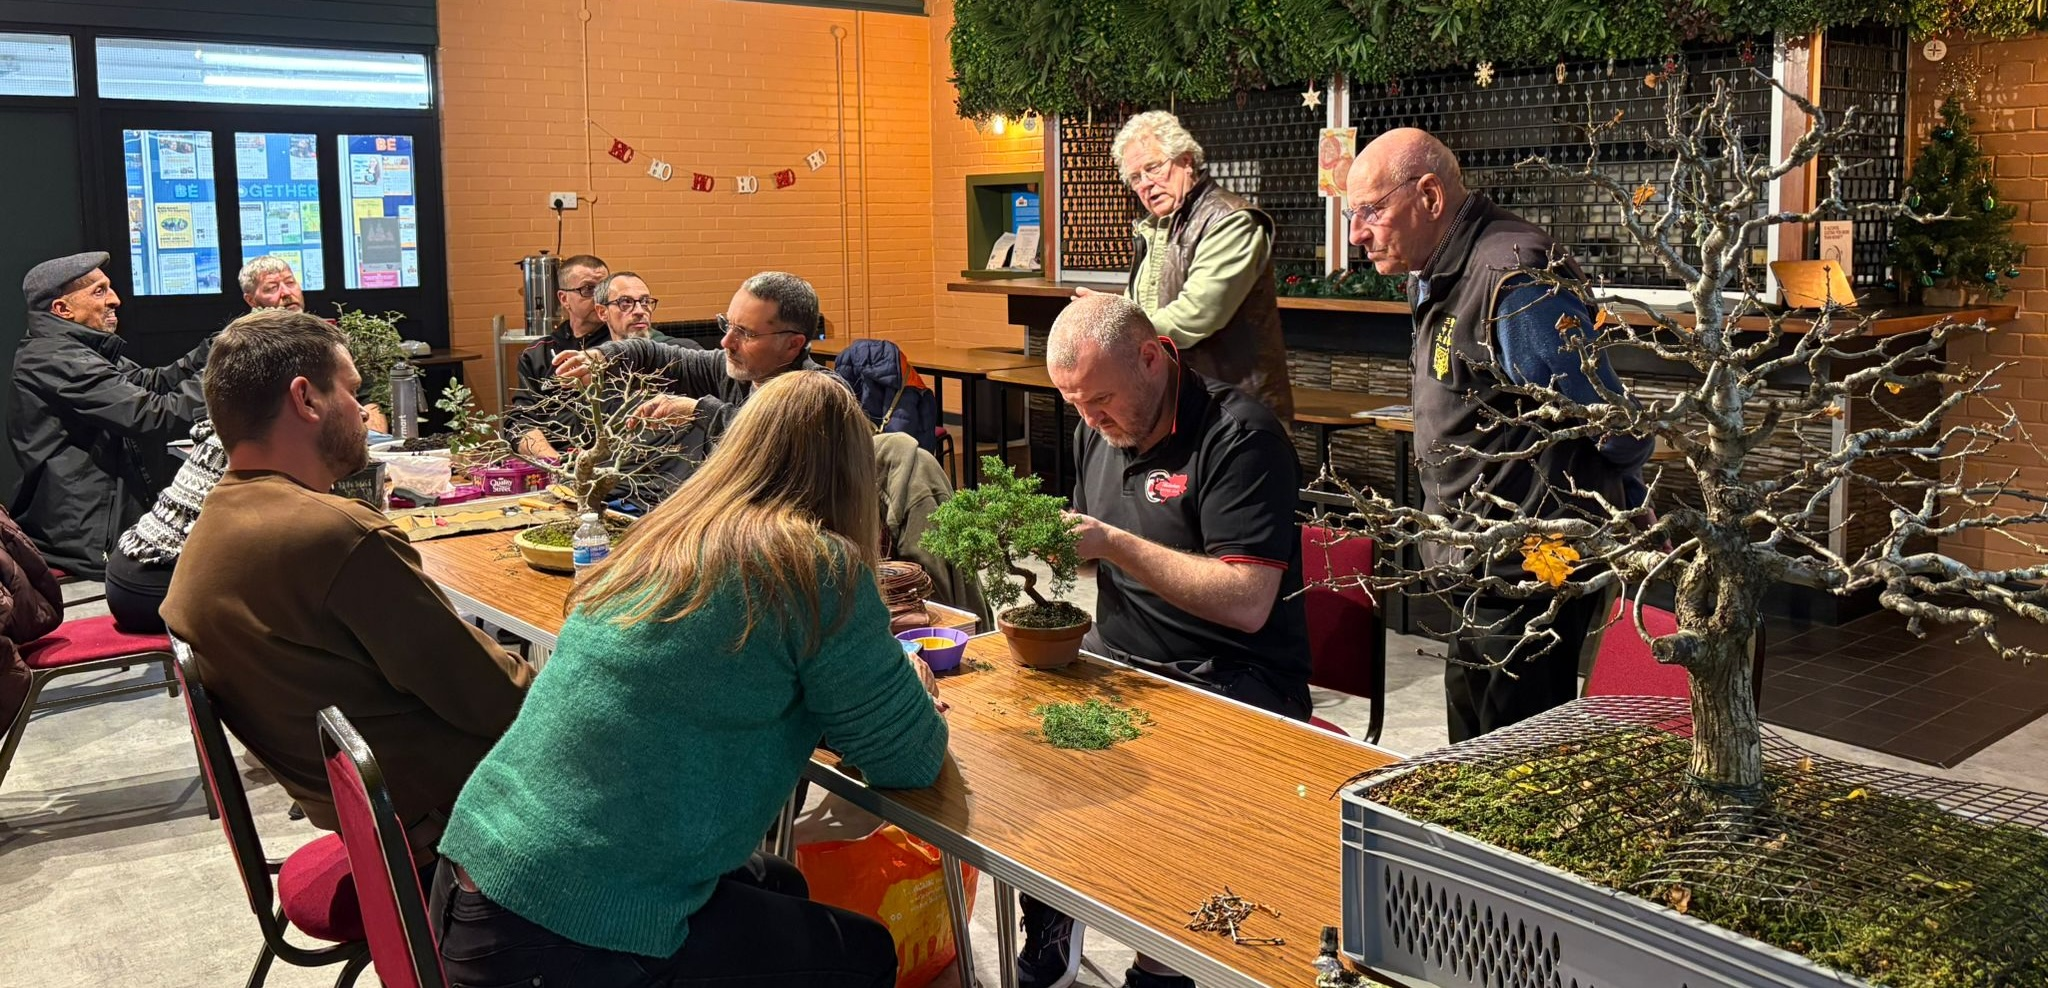
\includegraphics[width=1.0\columnwidth]{2025_12/res/editorial_december},\centerline{\emph{Members embracing festive spirit while working on their trees.}}]
%\end{window}
%\vspace*{-1em}
%\closearticle
%\clearpage